\documentclass{article}
\usepackage{xeCJK}
\usepackage[utf8]{inputenc}
\usepackage{graphicx}
\usepackage{soul}
\usepackage{caption}
\usepackage[utf8]{inputenc}
\usepackage{amsmath}
\usepackage[dvipsnames]{xcolor}
\DeclareMathOperator*{\argmax}{arg\,max}
\DeclareMathOperator*{\argmin}{arg\,min}

\title{Estimation by direct maximization of the likelihood}
\author{Yun-Hsiang Chan}
\date{June 2021}

\begin{document}

\maketitle

\section*{I. Introduction}
Previously, we know that the likelihood of an HMM is given by 
$$L_T = Pr(X^{(T)} = x^{(T)}) = \delta P(x_1) \Gamma P(x_2) ... \Gamma P(x_T)1')$$
where $\delta$ is the initial distribution and $P(x)$ the $m \times m$ diagonal matrix with ith diagnoal element the state-dependent probability or density $p_i(x)$. \\
\\
In principle, we can there compute $L_T = \alpha_T 1'$ recursively via
$$\alpha_1 = \delta P(x_1)$$
and,
$$\alpha_t = \alpha_{t_1} \Gamma P(x_t) \text{, for } t = 2, 3, ..., T$$
\\
If the Markov Chain is assumed stationary ($\delta = \delta \Gamma$), we can choose to use instead, 
$$\alpha_0 = \delta$$
and,
$$\alpha_t = \alpha_{t-1}\Gamma P(x_t) \text{, for } t = 1, 2, ..., T$$
\\
We shall first consider the staionary case. \\
\\
The number of operations involved is of order $Tm^2$, making the evaluation of the likelihood quite feasible even for large $T$. Parameter estimation can therefore be performed by numerical maximization of the likelihood with respect to the parameters. \\
\\
\textbf{Problem:}\\
When parameters are estimated in this ways, the main problems are\\
1. numerical underflow \\
2. constraints on the parameters \\
3. multiple local maxima in the likelihood function \\
\\
In this chapter, we will discuss how to overcome these problems, in order to arriave at a general strategy for computing MLEs. Then we discuss the estimation of standard errors for parameters.

\section*{II. Scaling the likelihood computation}

In the case of discrete state-dependent distributions, the elements of $\alpha_t$, being made up of products of probabilities become progressively smaller as $5$ increases, and are eventually rounded up to zero. In fact, with probability 1 the likelihood approaches 0 exponentially fast. \\
\\
Since the likelihood is a product of matrices, not of scalars, it is not possible to circumvent numerical underflow simply by computing the log of the likelihood as the sum of logs of its factors. In this respect, the computation of the likelihood of an independent mixture model is simpler than that of an HMM. \\
\\
To solve the problem, suppose we wish to compute $log(p+q)$, where $p > q$. Write, $log(p+q)$ as
$$log p + log(1+ q/p) = log p + log(1 + exp(\bar{q} - \bar{p}))$$
where $\bar{p} = log p$ and $\bar{q} = log q$. Then the function $log(1+e^x)$ is then approximated by interpolation from a table of its value. \\
\\
\textbf{Solution:}\\
Compute the logarithm of $L_T$ by using a strategy of scaling the vector of forward probabilities $\alpha_t$. \\
Effectively, we scale the vector $\alpha_t$ at each time $t$ so that its elements add to $1$, keeping track of the sum of the logs of the scale factors thus applied. \\
\\
Define, for $t = 1, ..., T$, the vector
$$\phi_t = \alpha_t / w_t$$
where $w_t = \sum_i \alpha_t(i) = \alpha_t 1'$. First, we note certain immediate consequences of the definitions of $\phi_t$ and $w_t$:
\begin{align}
w_0 = \alpha_0 1' & = \delta 1' = 1' \\
\phi_0 & = \delta\\
w_t \phi_t & = w_{t-1} \phi_{t-1} \Gamma P(x_t) \\
L_T = \alpha_T 1' & = w_T (\phi_T 1') = w_T \\
\end{align}
Hence,
$$L_T = w_T = \Pi_{t=1}^T (w_t / w_{t-1})$$
$$w_t = w_{t-1} (\phi_{t-1} \Gamma P(x_t) 1')$$
and so we conclude that
$$log L_T = \sum_{t=1}^T log(w_t / w_{t-1}) = \sum_{t=1}^T log(\phi_{t-1} \Gamma P(x_t) 1')$$
\\
The computation of the log-likelihood is summarized below in the form of an algorithm. Note, $\Gamma$ and $P(x_t)$ are $m \times m$ matrices, $v$ and $\phi_t$ are vectors of length $m$, $u$ is a scalr, and $l$ is the scalar in which the log-likelihood is accumulated.
\begin{align}
    \phi_0 \leftarrow \delta & ; l \leftarrow 0 \\
    \text{for } t  &= 1, 2, ... T \\
    v & \leftarrow \phi_{t-1} \Gamma P(x_t) \\
    u & \leftarrow v 1' \\
    l & \leftarrow l + log u \\
    \phi_t & \leftarrow v / u \\
    \text{return } & l
\end{align}
The required log-likelihood $log L_T$ is then given by the final value of $l$. The scale factor $w_t$ could be chosen instead to be the largest element of the vector being scaled, or the mean of its elements. \\
\\
The algorithm is easily modified to compute the log-likelihood without assuming stationarity of the Markov chain. With $\delta$ denoting the initial distribution, the more general algorithm is,
\begin{align}
    w_1 \leftarrow \delta P(x_1) 1' ; \phi_1  & \leftarrow \delta P(x_1) / w_1 ; l \leftarrow log w_1 \\
    \text{for } t = 2, 3, ..., T & \\
    v & \leftarrow \phi_{t-1} \Gamma P(x_t) \\
    u & \leftarrow v 1' \\
    l & \leftarrow l + log u \\
    \phi_t & \leftarrow v / u \\
    \text{return } l \text{                        } &
\end{align}
\\
The following code (Figure 1) implements this last version of the algorithm in order to compute the log-likelihood of observations $x_1, ..., x_T$ under a Poisson-HMM with at least two states, transition probability matrix $\Gamma$, vector of state-dependent means $\lambda$, and initial distribution $\delta$. \\
\begin{figure}
    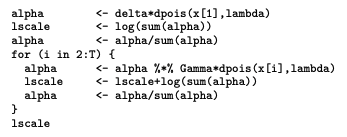
\includegraphics[width = 10cm]{algo.png}
    \caption{log-likelihood computation algorithm in R}
\end{figure}

\section*{III. Maximization of the likelihood subject to constraints}

The elements of HMM are always subject to non-negativity and other constraints. In particular, the row sums of $\Gamma$ equal 1. \\
\\
Estimates parameters should also satisfy such constraints. Thus, when maximizing the likelihood we need to slove a constrained optimization problem, not an unconstrained one. \\
\\
In general, there are two groups of constraints: \\
\textbf{1. apply to the parameters of the state dependent distributions} \\
\textbf{2. apply to the parameters of the Markov chain} \\
\\
For example, in the case of Poisson-HMM, the relevant constraints are: \\
- the means $\lambda_i$ of the state-dependent distributions must, for $i = 1, ..., m$, be non-negative. \\
- the rows of the transition probability matrix $\Gamma$ must add to 1, and all the parameters $\gamma_{ij}$ must be non-negative. \\
\\
Here are some constraints can be imposed by making transformations.

\subsection*{1. transformations of the parameters $\lambda_i$}
Define $\eta_i = log \lambda_i$, for $i = 1, ..., m$, then $\eta_i \in R$. \\ 
\\
After we have maximized the likelihood with respect to the unconstrained parameters, the constrained parameter estimates can be obtained by transforming back, $\hat{\lambda}_i = \text{exp } \hat{\eta_i}$.

\subsection*{2. reparameterization of the matrix $\Gamma$}
This requires more work but can be accomplished quite elegantly. \\
\\
Note that $\Gamma$ has $m^2$ entries but only $m(m-1)$ free parameters, as there are $m$ row-sum constraints. 
$$\sum_{j=1}^m \gamma_{ij} = 1, \text{($i = 1, ..., m$)}$$
\\
One possible transformation between the $m^2$ constrained probabilities $\gamma_{ij}$ and $m(m-1)$ constrained real numbers $\tau_{ij}, i \neq j$. \\
\\
1. Define a $m \times m$ matrix, with all diagnoal elements missing and others are corresponding to $\tau_{ij}$. \\
2. Now let $g: R \rightarrow R^+$ be a strictly increasing function, for example, $g(x) = e^x$. \\
3. Define \\
\[ v_{ij} = \begin{cases}
    g(\tau_{ij}) & \text{for $i \neq j$} \\
    1 & \text{for $i = j$}
\end{cases} \]
We then set $\gamma_{ij} = v_{ij} / \sum_{k=1}^m v_{ik}$ (for $i, j = 1, 2, ..., m$) and $\Gamma = (\gamma_{ij})$. \\
\\
We shall refer to the parameters $\eta_i$ and $\tau_{ij}$ as \textbf{working parameters}, and to the parameters $\lambda_i$ and $\tau_{ij}$ as \textbf{natural parameters}. 
\subsection*{Together}
Using above transformations of $\Gamma$ and $\lambda$, we can perform the calculation of the likelihood-maximizing parameters in \textbf{two steps}. \\
\\
1. Maximize $L_T$ with respect to the working parameters $T = \{\tau_{ij}\}$ and $\eta = \{(\eta_1, ..., \eta_m)\}$. They are all unconstrained. \\
\\
2. Transform the estimates of the working parameters to estimates of the natural parameters:
$$\hat{T} \rightarrow \hat{\Gamma}, \hat{\eta} \rightarrow \hat{\lambda}$$
\\
Consider $\Gamma$ for the case $g(x) = e^x$ and general $m$. Here we have 
$$\gamma_{ij} = \frac{exp(\tau_{ij})}{1 + \sum_{k \neq i} exp(\tau_{ik})}$$
and the diagonal elements of $\Gamma$ follow from the row sums of 1. THe transofrmation in the opposite direction is 
$$\tau_{ij} = log(\frac{\gamma_{ij}}{1 - \sum_{k \neq i} \tau_{ik}}) \text{, for } i \neq j$$
This generalization of the logit and inverse logit transforms has long been used in the context of compositional data. The code below (Figure 2) is an example of transform natural parameters to working and vice versa. \\
\begin{figure}
    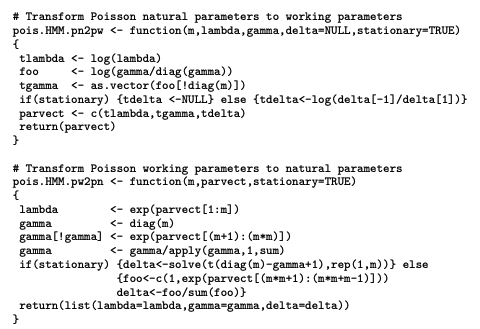
\includegraphics[width = 10cm]{code for transformation.png}
    \caption{transform natural parameters to working in R}
\end{figure}

\section*{IV. Other problems}
\subsection*{Multiple maxima in the likelihood}
The likelihood of an HMM is a complicated function of the parameters and frequently has several local maxima. \\
\\
There is no simple method of determining in genereal whether an algorithm has reached the global maximum, even if we apply the main alternative method of estimation, the EM algorithm. \\
\\
A sensible strategy is therefore to use a range of starting values for the maximization, and to see whether the same maximum is identified in each case. 

\subsection*{Starting values for the iterations}
It is less easy to guess values for the transition probabilities $\gamma_{ij}$. One strategy is to assign a common starting value to all the off-diagonal transition probabilities. \\
\\
A consequence of such a choice is that the corresponding stationary distribution is uniform over the states. Choosing good starting values for parameters tends to steer one away from numerical instability. 

\subsection*{Unbounded likelihood}
It may happen that the likelihood is unbounded in the vicinity of certain parameters combinations, like we state before. We can overcome it by maximizing the discrete likelihood instead of the joint density. 

\section*{V. Example: earthquakes}

See textbook. 

\section*{VI. Standard errors and confidence intervals}
Relatively little is known about the properties of the maximum likelihood estimators of HMMs. To exploit these results, one requires estimates of the variance-covariance matrix of the estimators of the parameters. \\
\\
There are \textbf{two ways} for estimates: \\
1. estimate the standard errors from \textbf{Hessian of the log-likelihood at the maximum} \\
- cons: some of the parameters are on the boundary of their parameter space, which occurs quite often when HMMs are fitted. \\
\\
2. \textbf{parametric bootstrap} \\
- pros: easy to code \\
- cons: computations are time-consuming

\subsection*{1. Standard errors via the Hessian}
In order to estimate the standard errors of the MLEs of an HMM, use the approximate Hessian of minus the log-likelihood at the minimum. We can invert it and so estimate the asymptotic variance-covariance matrix of the estimators of the parameters. \\
\\
A problem is that, if the parameters are transformed, the Hessian available will be that which referes to the working parameters $\phi_{i}$, not the original, more readily interpretable, natural parameters $\theta_i$. \\
\\
The situation is therefore that we have, at the minimum of $-l$, the Hessian with respect to the working parameters, 
$$H = -(\frac{\partial^2 l}{\partial \phi_i \partial \phi_j})$$
but what we really need is the Hessian with respect to the natural parameters, 
$$G = - (\frac{\partial^2 l}{\partial \theta_i \partial \theta_j})$$
There is, howevere, the following relationship between the two Hessians at the minimum:
$$H = MGM' \text{, and } G^{-1} = M' H^{-1} M$$
where $M$ is defined by $m_{ij} = \partial \theta_j / \partial \phi_i$. Then we can use $G^{-1}$ to find standard errors for the natural parameters. \\
\\
An alternative route to the standard errors with respect to the natural parameters wihich often works well, and is less laborious, is: \\
1. Find the MLE by solving the constrained optimiazation problem \\
2. Rerun the optimization without constraints, starting at or very close to the MLE. \\
\\
If the resulting estimate is the same as the MLE already found, the corresponding Hessian then directly supplies the standard errors with respect to the natural parameters. \\
\\
But if one is to make a normality assumption and base a confidence interval on it, such a normality assumption is more likely to be reasonable on the working-parameter scale than on the constrained natural-parameter scale. 

\subsection*{2. Recursive computation of the Hessian}

An alternative method of computing the Hessian, is the forward algorithm $\alpha_t = \alpha_{t-1} \Gamma P(x_t)$ in a form which incorporates automatic or 'natural' scaling, and then extend that approach in order to compute its Hessian and gradient with respect to the natural parameters, those we have denoted above by $\theta_i$. \\
\\
Although this may be a more effecient and accurate method, it doesn't solve the fundmental problem that the use of the Hessian to compute standard errors is unreliable if some parameters are on or near the boundary of their parameter space.

\subsection*{3. Bootstrap standard errors and confidence intervals}
The idea of the \textbf{parametric bootstrap} is to assess the properties of the model with parameters $\Theta$ by using those of the odel with parameters $\hat{\Theta}$. \\
\\
1. Fit the model i.e. compute $\hat{\Theta}$ \\
\\
2. (a) Generate a sample, called bootstrap sample of observations from the fitted model, i.e. model with parameters $\hat{\Theta}$. The length should be the same as the original number of observations. \\
\\
2. (b) Estimate the parameter $\Theta$ by $\hat{\Theta}^*$ for the bootstrap samples. \\
\\
2. (c) Repeat steps (a) and (b) B times, and record the values $\hat{\Theta}^*$ \\
\\
The variance-covariance matrix of $\hat{\Theta}$ is then estimated by the sample variance-covariance matrix of the bootstrap estimates $\hat{\Theta}^*(b)$, $b = 1, 2, ..., B$
$$\hat{\text{Var-Cov}}(\hat{\Theta}) = \frac{1}{B-1} \sum_{b=1}^B (\hat{\Theta}^* (b) - \hat{\Theta}^* (.))' (\hat{\Theta}^* (b) - \hat{\Theta}^* (.))$$
where $\hat{\Theta}^*(.) = B^{-1} \sum_{b=1}^B \hat{\Theta}^* (b)$ \\
\\
The parametric bootstrap requires code to generate realizations from a fitted model, and can be used to estimate confidence intervals directly. 

\section*{VII. Example: the parametric bootstrap applied to three-state model for the earthquakes data}

See textbook.










\end{document}